\chapter{相关工作}

\section{生成式对抗网络}

\subsection{生成式对抗网络的概念}

基于生成式对抗网络~\cite{GANs}的生成模型极大的提升了图片生成的真实度~\cite{BigGANs,StyleGAN}。生成式对抗网络由生成器和判别器组成,生成器负责将隐变量(一般是从高斯分布采样的噪声)映射为生成的图像,判别器是一个二分类器,用于区分生成图像与真实图像。生成器和判别器以一种对抗的方式交替训练,这也是生成式对抗网络最核心的贡献。

虽然生成式对抗网络已经能够生成足够真实的图像,却需要很长的训练时间,以StyleGAN为例,在单Tesla V100显卡上训练需要接近70天!等人在2021年推出了一种轻量级GANs,得益于器搞笑的网络结构和数据增广策略,只需要几个小时就能在单卡上完成训练。生成效果如图~\ref{LWGAN}所示,可以看到这种轻量级GANs在生成质量上不如BigGANs、StyleGAN等重量级网络,但考虑到个人和科研机构往往计算资源有限,因此这类轻量级GANs仍有非常重要的现实意义。

\begin{figure}
    \centering
    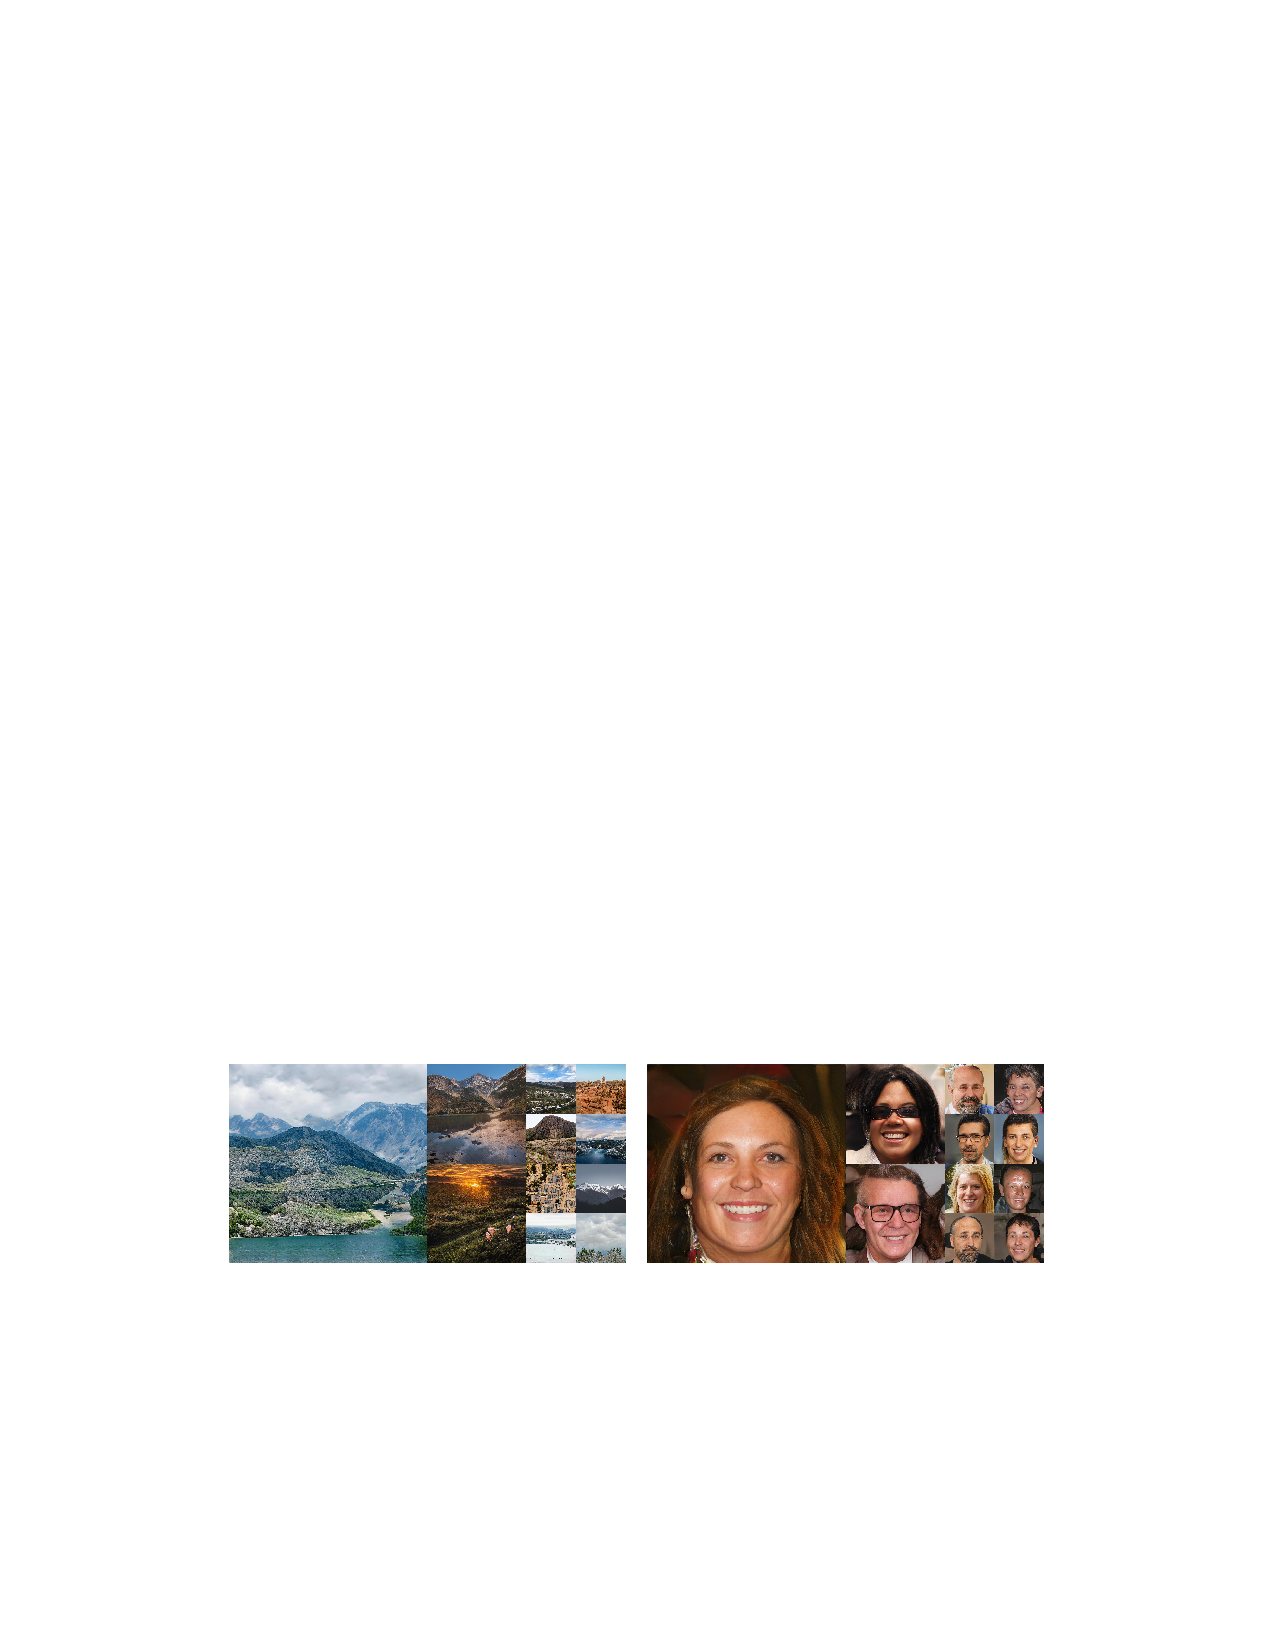
\includegraphics[width=\textwidth]{figures/LWGAN.pdf}
    \caption{轻量级GANs在1024x1024分辨率下的生成效果,可以看到这种轻量级GANs在生成质量上不如BigGANs、StyleGAN等重量级网络,但考虑到个人和科研机构往往计算资源有限,因此这类轻量级GANs仍有非常重要的现实意义。}
    \label{LWGAN}
\end{figure}

\subsection{生成式对抗网络的训练}

生成器和判别器以一种对抗的方式交替训练,我们以先优化判别器为例,介绍GANs的训练流程。

在每次模型迭代中,我们先以公式~\ref{step_D}优化判别器,注意此时我们固定生成器的权重不变。

\begin{equation}
    \max _{D} V(D, G, R) = \mathcal{L}_{GAN}(G, D) + \lambda \mathcal{L}_{Reg}(G, R),
    \label{step_D}
\end{equation}

然后,我们以公式~\ref{step_G}优化生成器,同样的,此时我们固定判别器的权重不变。

\begin{equation}
    \min _{G} V(D, G, R) = \mathcal{L}_{GAN}(G, D) + \lambda \mathcal{L}_{Reg}(G, R),
    \label{step_G}
\end{equation}

将公式~\ref{step_D}和~\ref{step_G}结合起来,我们就得到了如公式~\ref{overall}所示的GANs总损失。

\begin{equation}
    \min _{G} \max _{D} V(D, G, R) = \mathcal{L}_{GAN}(G, D) + \lambda \mathcal{L}_{Reg}(G, R),
\end{equation}

重复上述步骤,直到生成器生成的图像对人来说足够真实,生成图像的真实度也可以FID~\cite{FID}等度量方法辅助判断。与其他机器学习模型不同,生成器和判别器的损失并不能直接表明模型的好坏,而是需要我们观察生成图像的质量。

\section{图片空间编辑}

图像空间编辑指将输入图像从原风格转换为目标风格(风格转换)或从原图像域转换为目标图像域(图像转换)。 随着深度学习的发展,神经网络风格迁移(neural sytle transfer)~\cite{transfer0,transfer1,transfer2}已经成为风格迁移的主流方法。 风格迁移侧重于不同的艺术风格间的转换,而图像转换\cite{i2i0,i2i1,i2i2,cyclegan} 解决了更一般的图像域转换问题。
大多数这些方法~\cite{yu2018super,lu2018attribute} 很难同时编辑多个属性并精确控制生成图像中的属性程度。

\section{隐空间编辑}

在GANs发展的早期,Alec Radford等人就在\cite{DCGAN}中发现GANs的隐空间中通常包含有语义意义的向量算法,例如,隐空间中存在能为人脸添加微笑或眼镜的方向。我们称这类通过隐空间向量运算实现图像编辑发方法为隐空间编辑方法,区别与上文提到的图像空间编辑方法,后者是对图像直接的转换。

由于隐空间编辑使图像编辑更加简单,因此近些年来这类方法收到越来越到的关注。从隐空间编辑的监督方式来看,隐空间编辑方法分为有监督、无监督、自监督或半监督的方法。

\begin{enumerate}
\item 有监督的隐空间编辑方法采用明确的人工监督来识别潜在空间中的可解释方向,如Yujun Shen等人~\cite{interfacegan}使用在CelebA数据集~\cite{celeba}上预训练的二分类器来预测人脸属性。然后使用该分类器为生成的图像及对应的隐变量生成伪标签。基于这些伪标签,可以在隐空间空间中构建分类超平面,该超平面的法线即为相应属性变化的方向。

\item 无监督通过学习一组语义上不同的方向~\cite{icml2020} 或基于主成分分析(PCA)~\cite{harkonen2020ganspace}识别潜在的的语义方向。这些方法可能会找到有意义的方向,但其结果是不可预测的,并且需要人工解释,这导致了非监督的隐空间编辑方法难以指定所需的属性方向。

\item 自监督方法~\cite{steer,variation} 通过使用简单的几何变换(例如旋转和缩放)增加数据来搜索可解释的方向,这限制了这些方法搜索复杂属性的能力。半监督方法~\cite{nie2020semi} 调查了有限监督的影响,这很难同时进行良好的解开和良好的编辑多个属性。
\end{enumerate}

以上方法均是在预训练的GANs的隐空间中搜索语义方向,不可避免收到预训练GANs的影响,由于GANs在训练时没有受到语义属性的约束,其隐空间必然存在语义耦合现象。这导致现有的隐空间编辑的方法在改变某一属性时,不可避免地会改变其他的属性。    

\section{多模态图像转换}

在图像处理、计算机视觉和计算机图形学的许多应用中,越来越依赖于多模态医学图像。例如精准医学,脑部核磁共振中存在T1、T1Gd、T2和T2-FLAIR四种模态~\cite{drevelegas2011imaging}。医生希望结合完整的多模态医学图像来做出更精确的诊断,但受限于某些实际限制(例如,受限的医疗条件、扫描时间不足以及成本/支出/资源等限制)可能导致成像模态存在系统误差,甚至造成部分模态的缺失~\cite{tanenbaum2017synthetic}。这些不可用的图像可能会导致医生决策出现偏差。

Dongwook Lee等人提出的CollaGAN~\cite{collagan}是第一篇将GANs用于多模态图像。与CycleGAN,Pix2Pix等单模态图像转换方法只能输入一种模态的图像不同,CollaGAN针对多模态图像转换提出了多重循环一致损失(Multiple cycle consistency loss),通过一个GANs模型解决了多模态间模态转换的问题。Bing Cao等人提出的Auto-GAN~\cite{AutoGAN}则更关注多模态场景下训练稳定性的问题,作者提出使用自表示网络在训练过程中对生成器网络特征图的表示进行引导,这里的自表示网络由一个简单的自编码器实现。

CollaGAN和Auto-GAN均使用单个模型在一定程度上解决了多模态图像转换的问题,但都没有在训练过程中对模态间的一致性和互补性进行约束。

\section{本章小结}

在本章节我们总结生成式对抗网络,图片空间编辑、隐空间编辑和多模态图像转换的原理、应用和进展,重点梳理了隐空间编辑和多模态图像现有方法的优势与不足,为后续本文解决方案的提出奠定了基础。
